\section{滑动窗口优化}

通常在实现SLAM算法时,需要在算法的精度和性能两者中做出权衡。完整的集束优化(full bundle adjustment),包括对所有历史状态的所有观测,虽然可以获得最优的状态估计,但其计算代价往往是难以接受的。在一些对性能要求高的应用场景,例如实时增强现实应用和自动驾驶应用中,算法的性能往往决定了它的可用性。相对而言,这一类应用的精度要求就可以被适当放宽。

随着对实时的、高效SLAM算法需求的日益增加,一些致力于在保证一定精度的前提下降低计算代价的集束优化算法应运而生,其主要通过两种策略来减少算法的计算量。一种是针对应用场景的特点减小集束优化问题的规模,具体来说有以下几种:

\begin{itemize}
  \item 减少变量的个数:只保留状态变量,而不保留三维点变量,如Pose Graph优化算法\citep{lu1997globally};
  \item 基于固定历史时间窗口(fixed-lag\citep{dong2011motion}):只估计最近一段固定时间内的历史状态;
  \item 基于历史状态窗口(sliding-window\citep{mouragnon2006real}):只估计最近的数个历史状态;
  \item 基于关键帧(keyframe):只估计一部分选定的携带了足够信息的历史状态,如RKSLAM\citep{liu2016robust}、OKVIS\citep{leutenegger2015keyframe}等。
\end{itemize}

\begin{figure}[htbp]
  \centering
  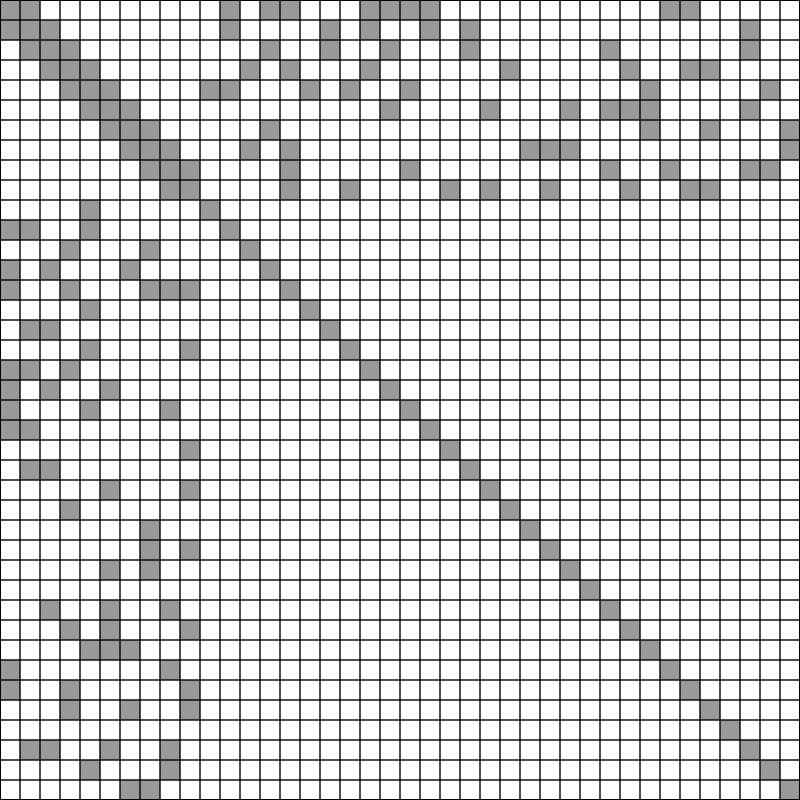
\includegraphics[width=.5\textwidth]{./figs/sparse_matrix.png}
  \caption{一般的稀疏矩阵结构}
  \label{fig:sparse_matrix}
\end{figure}

当然,以上的方法通常也可以结合使用。另一种策略是通过深入分析集束优化问题的特点,做针对性优化,减少冗余的计算。集束优化问题通常具有非常特殊的性质,合理利用这些性质,可以帮助我们更高效地求解SLAM系统的状态估计。比如,在SLAM系统中,通常需要求解的三维点变量的数量要远大于状态变量的数量,而且通常状态约束(constraints)集中在状态与状态之间、状态与三维点之间。这就导致集束优化构建的标准方程(normal equation)具有特别的稀疏结构,如图\ref{fig:sparse_matrix}所示:

另外,在线的集束优化中,通常只有较新加入的变量会发生比较大的变动,旧的变量由于经过持续的优化而变动很小。可以利用这种局部的性质,只对少部分变量进行更新,从而减少集束优化的计算量。

\subsection{条件状态估计}

\subsection{边缘状态估计}

前面提到,在删去被舍弃的三维点变量之前,要先以边缘化的方式将其信息保留下来,即得到剩余变量的边缘概率分布。显然,位姿图优化是对完整集束优化的近似,原因在于消去三维点变量后,三维点变量的信息被“永远”定在了发生边缘化的时刻,而后续即使状态变量发生了改变,其与旧的三维点的之间的信息由于已经被编码进了相对位姿约束而不能再改变,这就造成了所谓的“信息不一致(inconsistency)”,从而引入一些不必要的误差。为了解决信息一致性的问题,部分SLAM算法引入了FEJ技术(first estimate jacobian)\citep{huang2008analysis,li2012improving}。
